\documentclass{article}\usepackage[]{graphicx}\usepackage[]{color}
%% maxwidth is the original width if it is less than linewidth
%% otherwise use linewidth (to make sure the graphics do not exceed the margin)
\makeatletter
\def\maxwidth{ %
  \ifdim\Gin@nat@width>\linewidth
    \linewidth
  \else
    \Gin@nat@width
  \fi
}
\makeatother

\definecolor{fgcolor}{rgb}{0.345, 0.345, 0.345}
\newcommand{\hlnum}[1]{\textcolor[rgb]{0.686,0.059,0.569}{#1}}%
\newcommand{\hlstr}[1]{\textcolor[rgb]{0.192,0.494,0.8}{#1}}%
\newcommand{\hlcom}[1]{\textcolor[rgb]{0.678,0.584,0.686}{\textit{#1}}}%
\newcommand{\hlopt}[1]{\textcolor[rgb]{0,0,0}{#1}}%
\newcommand{\hlstd}[1]{\textcolor[rgb]{0.345,0.345,0.345}{#1}}%
\newcommand{\hlkwa}[1]{\textcolor[rgb]{0.161,0.373,0.58}{\textbf{#1}}}%
\newcommand{\hlkwb}[1]{\textcolor[rgb]{0.69,0.353,0.396}{#1}}%
\newcommand{\hlkwc}[1]{\textcolor[rgb]{0.333,0.667,0.333}{#1}}%
\newcommand{\hlkwd}[1]{\textcolor[rgb]{0.737,0.353,0.396}{\textbf{#1}}}%
\let\hlipl\hlkwb

\usepackage{framed}
\makeatletter
\newenvironment{kframe}{%
 \def\at@end@of@kframe{}%
 \ifinner\ifhmode%
  \def\at@end@of@kframe{\end{minipage}}%
  \begin{minipage}{\columnwidth}%
 \fi\fi%
 \def\FrameCommand##1{\hskip\@totalleftmargin \hskip-\fboxsep
 \colorbox{shadecolor}{##1}\hskip-\fboxsep
     % There is no \\@totalrightmargin, so:
     \hskip-\linewidth \hskip-\@totalleftmargin \hskip\columnwidth}%
 \MakeFramed {\advance\hsize-\width
   \@totalleftmargin\z@ \linewidth\hsize
   \@setminipage}}%
 {\par\unskip\endMakeFramed%
 \at@end@of@kframe}
\makeatother

\definecolor{shadecolor}{rgb}{.97, .97, .97}
\definecolor{messagecolor}{rgb}{0, 0, 0}
\definecolor{warningcolor}{rgb}{1, 0, 1}
\definecolor{errorcolor}{rgb}{1, 0, 0}
\newenvironment{knitrout}{}{} % an empty environment to be redefined in TeX

\usepackage{alltt}

\usepackage[english]{babel}
\usepackage{graphicx}
\usepackage{fancyref}
\usepackage{hyperref}
\usepackage[scale=2]{ccicons}
\usepackage{url}
\usepackage{fancyhdr}



\title{Exercises linear modelling}
\IfFileExists{upquote.sty}{\usepackage{upquote}}{}
\begin{document}





\subsection{Exercises}

Below, variables are printed in \textbf{bold}. For each research statement, identify which variable is the dependent variable, and which variable is the independent variable.

\begin{enumerate}

\item The effect of \textbf{income} on \textbf{health}
\item \textbf{Stock value} is affected by \textbf{inflation}
\item \textbf{Size} is influenced by \textbf{weight}
\item \textbf{Shoe size} is predicted by \textbf{sex}
\item The less you \textbf{drink} the more \textbf{thirsty} you become
\item The more \textbf{calories} you eat, the more you \textbf{weigh}
\item \textbf{Weight} is affected by \textbf{food intake}
\item \textbf{Weight} is affected by \textbf{exercise}
\item \textbf{Food intake} is predicted by \textbf{time of year}
\item There is an effect of \textbf{exercise} on \textbf{heart rate}
\item \textbf{Inflation} leads to higher \textbf{wages}
\item \textbf{Unprotected sex} leads to \textbf{pregnancy}
\item \textbf{HIV-infection} is caused by \textbf{unprotected sex}
\item The effect of \textbf{alcohol intake} on \textbf{driving performance}
\item \textbf{Sunshine} causes \textbf{growth}


\end{enumerate}

Answers:

\begin{enumerate}

\item \textbf{income} independent, \textbf{health} dependent.
\item \textbf{Stock value} dependent, \textbf{inflation} independent
\item \textbf{Size} dependent, \textbf{weight} independent
\item \textbf{Shoe size} dependent, \textbf{sex} independent
\item \textbf{drink} independent, \textbf{thirsty} dependent
\item \textbf{calories} independent, \textbf{weigh} dependent
\item \textbf{Weight} dependent, \textbf{food intake} independent
\item \textbf{Weight} dependent, \textbf{exercise} independent
\item \textbf{Food intake} dependent, \textbf{time of year} independent
\item \textbf{exercise} independent, \textbf{heart rate} dependent
\item \textbf{Inflation} independent, \textbf{wages} dependent
\item \textbf{Unprotected sex} independent, \textbf{pregnancy} dependent
\item \textbf{HIV-infection} dependent, \textbf{unprotected sex} independent
\item \textbf{alcohol intake} independent, \textbf{driving performance} dependent
\item \textbf{Sunshine} independent, \textbf{growth} dependent


\end{enumerate}




\subsection{Exercises}

\begin{enumerate}
\item
For Figures \ref{fig:lm_4}, \ref{fig:lm_5} and \ref{fig:lm_6}, give the linear equations for the relationship between $x$ and $y$.


\begin{knitrout}
\definecolor{shadecolor}{rgb}{0.969, 0.969, 0.969}\color{fgcolor}\begin{figure}

{\centering 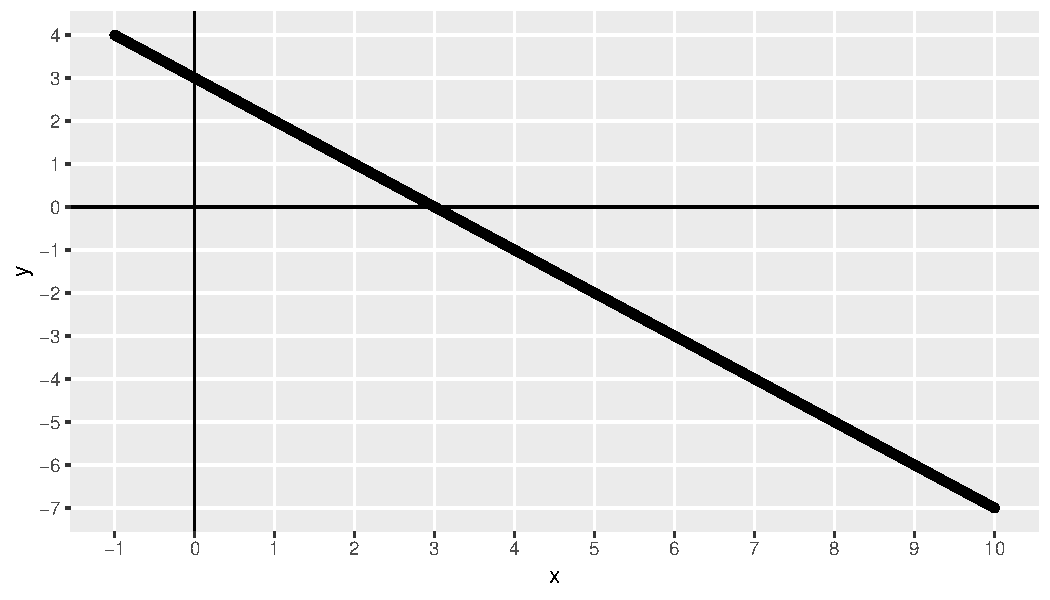
\includegraphics[width=\maxwidth]{figure/lm_4-1} 

}

\caption[Straight line example]{Straight line example.}\label{fig:lm_4}
\end{figure}


\end{knitrout}

\begin{knitrout}
\definecolor{shadecolor}{rgb}{0.969, 0.969, 0.969}\color{fgcolor}\begin{figure}

{\centering 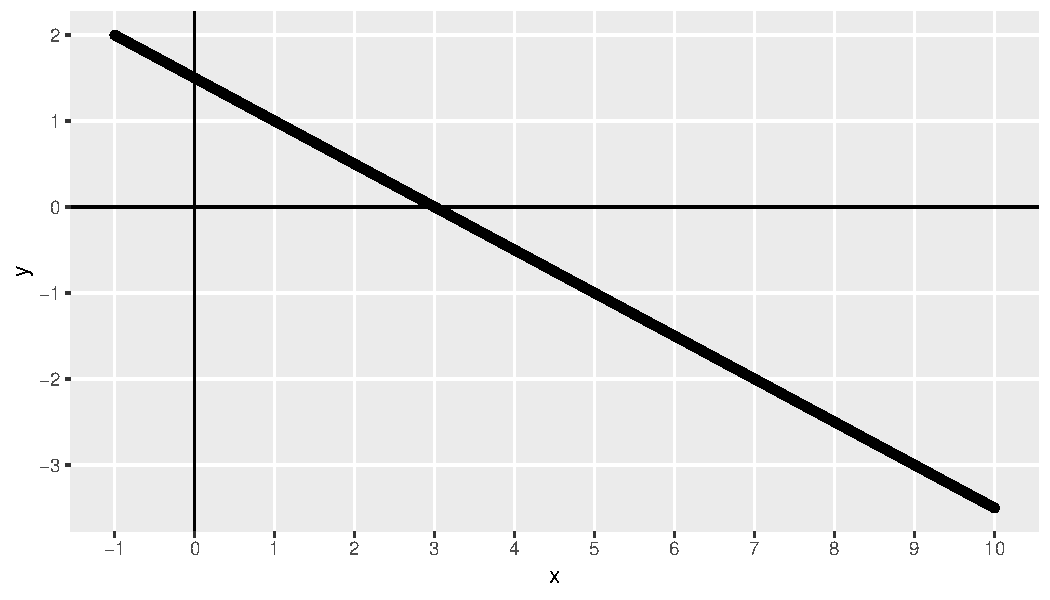
\includegraphics[width=\maxwidth]{figure/lm_5-1} 

}

\caption[Straight line example]{Straight line example.}\label{fig:lm_5}
\end{figure}


\end{knitrout}

\begin{knitrout}
\definecolor{shadecolor}{rgb}{0.969, 0.969, 0.969}\color{fgcolor}\begin{figure}

{\centering 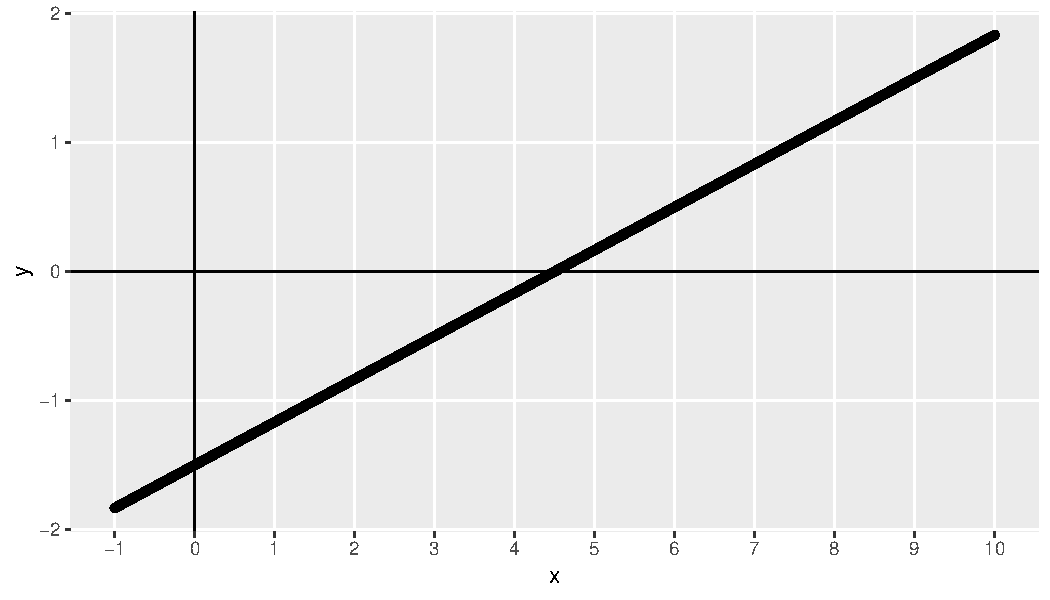
\includegraphics[width=\maxwidth]{figure/lm_6-1} 

}

\caption[Straight line example]{Straight line example.}\label{fig:lm_6}
\end{figure}


\end{knitrout}
\item
Try to sketch the straight line for the equation $y=1 - 2x$


\end{enumerate}


\subsection{Answers}

The equations are
\begin{enumerate}
\item
\begin{equation}
y = 3 - 1 x
\end{equation}
\item
\begin{equation}
y = 1.5 - 0.5 x
\end{equation}
\item
\begin{equation}
y = -2 + 0.33 x
\end{equation}
\item
The straight line for $y=1 - 2x$ is presented in Figure \ref{fig:lm_7}.

\end{enumerate}


\begin{knitrout}
\definecolor{shadecolor}{rgb}{0.969, 0.969, 0.969}\color{fgcolor}\begin{figure}

{\centering 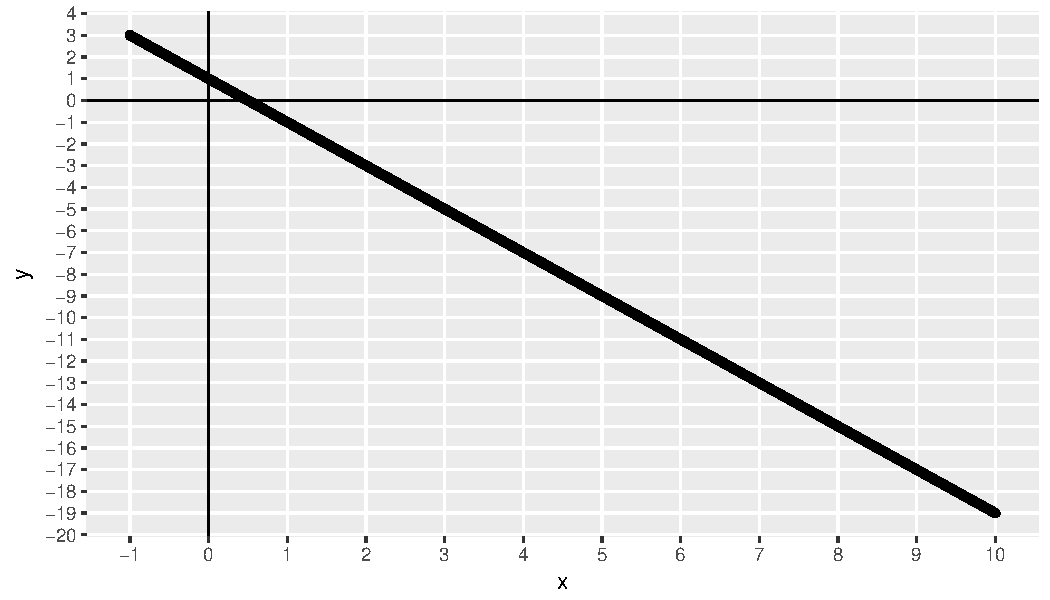
\includegraphics[width=\maxwidth]{figure/lm_7-1} 

}

\caption[Straight line with based on y=1-2x]{Straight line with based on y=1-2x.}\label{fig:lm_7}
\end{figure}


\end{knitrout}

% \subsection{Exercises}
%
% \begin{enumerate}
%
%
%
% <<lm_15, fig.height=4, echo=FALSE, fig.align='center', message=F, results="asis", warning=F>>=
% set.seed(123)
% area <- runif(10, 30, 120) %>% round(0)
% price <- rnorm(10, 0.9*area+80, 20) %>% round(0)
%
% tibble(Area=area, Price=price, PredictedPrice = " ", Residual=" ", SquaredResidual=" ") %>%
%         head() %>%
%         xtable(caption="Home prices.", label="tab:lm_15") %>%
%         print(include.rownames=F, caption.placement = "top")
%
% out.price <- lm(price ~ area , data=tibble(area, price))
% @
%
% \item In Table \ref{tab:lm_15} you find a small data set on the price of homes with dependent variable price in kEuros and independent variable area in square meters. The least squares regression equation turns out to be $price = out.price$coef[1]+ out.price$coef[2]\times area$. Add a third column with the expected prices based on the regression equation ($\hat{y}$. Put the difference between the observed price and the expected price in the fourth column ($e$). Then compute the squared residuals and put those in the fifth column ($e^2)$. Take the sum of the squared residuals: How large is sum of the squared residuals?
%
%
% \item See website \url{https://gallery.shinyapps.io/simple_regression/}, try to find the Least Squares regression line for the given data set by changing both intercept and slope. How large is the sum of the squared residuals for that optimal regression line?
%
%
% \item Do this exercice with one or more of your fellow students. Look at the data set plotted in Figure \ref{fig:lm_16}. Try to find the regression line with the lowest sum of squared residuals possible.
%
% <<lm_16,fig.height=4, echo=FALSE, fig.align='center', fig.cap='Plot of housing data.'>>=
% set.seed(1234)
% x <- runif(5, 30, 120) %>% round(0)
% y <- rnorm(5, area+80, 20) %>% round(0)
% y <- c(15, 20, 10, 10, 5)
% x <- x/10
%
% tibble(x, y) %>%
%         ggplot(aes(x, y)) +
%         geom_point() +
%         ylim(c(5,22))
%  out <- lm(y~x)
% @
%
%
% \end{enumerate}
%
% \subsection{Answers}
%
%
% \begin{enumerate}
%
% \item The predicted prices, the residuals and the squared residuals are displayed in Table \ref{tab:lm_17}. The sum of the squared residuals equals sum(out.price$residuals^2).
%
% <<lm_17, fig.height=4, echo=FALSE, fig.align='center', message=F, results="asis", warning=F>>=
% tibble(Area=area, Price=price, PredictedPrice = predict(out.price), Residual=out.price$residuals, SquaredResidual=out.price$residuals^2) %>%
%                 head() %>%
%                 xtable(caption="Home prices.", label="tab:lm_17") %>%
%                 print(include.rownames=F, caption.placement = "top")
% @
% \item
%
% \item The lowest sum of squared residuals is round(sum(out$residuals^2),0). This is the sum that you get with intercept round(out$coef[1],1) and slope round(out$coef[2],1).
%
% \end{enumerate}
%
%





% \subsection{Exercises}
%
% \begin{enumerate}
%
% \item The correlation between brain size and intelligence in 9-year-old children equals 0.30. Suppose the variance in brain size equals 45 and the variance in intelligence 225. Compute the covariance.
%
%
%
% \item The covariance between intelligence and extraversion equals 1. The variance of intelligence is 225 and the variance of extraversion is 9. What is the correlation?
%
%
%
%
% \item Suppose the correlation between intelligence and extraversion is 0.10. What does this mean?
%
%
%
% \item Suppose the correlation between intelligence and extraversion is -0.05. What does this mean?
%
%
%
%
% \item Suppose the correlation between intelligence and extraversion is 0.30. What is the regression slope if the variance of intelligence is 225 and the variance of extraversion is 9?
%
%
%
% \end{enumerate}
%
% \subsection{Answers}
%
% \begin{enumerate}
%
% \item
%
% \begin{equation}
% \sigma_{xy}= r_{xy} \times \sigma_x \sigma_y= 0.30 \times \sqrt{45}\times \sqrt{225}=round(0.30*sqrt(45)*15)
% \end{equation}
%
%
%
% \item
%
% \begin{equation}
% r_{xy}= \frac{\sigma_{xy}} { \sigma_x \sigma_y}= \frac{1} { \sqrt{225} \sqrt{9}}=round(1/(15*3),2)
% \end{equation}
%
% \item
% If you increase intelligence by 1 standard deviation, then extraversion increases with a tenth of a standard deviation.
%
% \item
% If you increase intelligence by 1 standard deviation, then extraversion increases with 0.05 standard deviations.
%
% \item
% The correlation is 0.30, so if you increase intelligence by one standard deviation (which is $\sqrt{225}=15$), extraversion increases by 0.30 standard deviations (which equals $0.30 \times \sqrt{9}=0.90$). Therefore, if you increase intelligence by 15 points, you increase extraversion by 0.90 points. Thus if you increase intelligence by 1 point, you increase extraversion by $0.90/15=round(0.9/15,2)$ points. The slope for the regression of extraversion on intelligence is therefore round(0.9/15,2).
%
%
% \end{enumerate}

\end{document}


